\documentclass[10pt]{article}
\usepackage{acl2014}
\usepackage[utf8]{inputenc}
\usepackage{times}
\usepackage{url}
\usepackage{amsmath}
\usepackage[natbib=true,backend=bibtex,style=authoryear,language=english]{biblatex}
\usepackage{lipsum}
\usepackage{latexsym}
\usepackage[normalem]{ulem}
\usepackage[ruled]{algorithm2e}
\usepackage[]{setspace}
\useunder{\uline}{\ul}{}
\usepackage{caption} 
\usepackage{lastpage}
\pagestyle{plain} 
\usepackage{graphicx}
\captionsetup[table]{skip=10pt}
\title{Intelligent Traffic Control}

\addbibresource{references.bib}
\AtBeginBibliography{\small}

\author{Thomas van den Broek, Vincent Van Driel, Zsolt Harsányi, Tonio Weidler\\
	Department of Data Science \& Knowledge Engineering\\
	Maastricht, The Netherlands\\
	\tt \small vincevandriel@gmail.com, thomasbuo@gmail.com,\\
	\tt \small zsharsany@gmail.com, uni@tonioweidler.de
}
  
\begin{document}

\maketitle
\begin{abstract}
\lipsum[1]
{{\it \bf Keywords:} traffic simulation; traffic control; strategies; linear programming; machine learning; realistic environment; IDM; MOBIL;}
\end{abstract}

\section{Introduction}
An intelligent traffic control system adjusts traffic in order to assure all people reach their destinations in the most optimal time and distance. These systems are important for the daily workings of major cities by alleviating traffic congestion and identifying problem areas.  It is important to constantly keep these systems updated to assure optimal performance and safety of the general public. With advancements in technology and artificial intelligence, new and more sophisticated strategies for traffic control become possible.

\subsection{Goal}
In this work, we aim to evaluate different traffic control strategies and compare their effect. We hope to identify the best working solutions to traffic jams and other occurrences (such as closing of roads/tunnels) in cities and to show their workings. We attempt to recreate a city's traffic flow in order to see how these systems would work in a realistic setting. Our simulation aims to model the dynamics of a realistic environment as close as possible within the scope of the project, so that the comparison is meaningful and provides valuable data regarding the potential application of the strategies.

Our main contributions are as follows:

\subsection{Approach}
Hence, in order to test the effect of different intelligent traffic control strategies, an appropriate simulation is required. For this purpose, we created a simulation environment which allows the incorporation of different such strategies into a dynamic traffic model. Maps are realised as undirected graphs in which vertices represent intersections and roads appear as edges between those. The simulation is \textit{microscopic}. That is, instead of globally controlling traffic (\textit{macroscopic}), the atomic parts of the simulation are locally controlled cars \citep[see also][]{krajzewicz2002sumo}. Driving behaviour is modelled using the time- and space-continuous \textit{Intelligent Driver Model} (IDM) \citep{treiber2000congested}. 

\subsection{Related Work}
\label{sec:related-work}
There has been extensive work on the simulation of traffic flow as well as the development of traffic control strategies. Following up on different approaches on modelling car following behaviour \citep[e.g.][]{gipps1981behavioural}, \citet{treiber2000congested} developed the influential Intelligent Driver Model for the simulation of urban traffic. Similarly to the former, it creates a collision free environment where cars mind the  spacial and time-wise gap to the leading vehicle. The SUMO package \citep{krajzewicz2002sumo, behrisch2011sumo} utilizes the model by \citep{gipps1981behavioural} in an extended version \citep{krauss1998microscopic} in a complex simulation software. In contrast to their research, this work uses the IDM. Hence, the simulation is time-continuous, rather than time-discrete.

Often utilizing such simulation environments for evaluation purposes, a lot of research exists investigating the strengths of different approaches to the automatic control of traffic signals or traffic lights. \citet{papageorgiou2003review} have reviewed such research and identified two key characteristics according to which strategies may be classified. They distinguish between \textit{fixed-time} and \textit{traffic-responsive} strategies, as well as \textit{isolated} and \textit{coordinated} strategies. Fixed-time strategies use historical data to determine (e.g. by optimization) static cycle lengths, while traffic-responsive strategies may use different techniques (e.g. heuristics or optimization algorithms) in order to derive optimal cycle lengths from real-time data that has to be measured in some way. Isolated strategies are focused on a single intersection, while coordinated strategies are able to communicate information between multiple intersections and thereby make potentially joint decisions. \citet{coll2013linear} categorize strategies into four categories. They also distinguish between fixed-time and traffic-responsive approaches, but additionally differentiate \textit{adaptive systems} that apply optimization techniques and \textit{predictive strategies} that use both online and off-line information in order to predict future arrivals at the intersection \citep{coll2013linear}. In this work, the focus will be laid on the former two categories, that is fixed-time and responsive. Nevertheless, one of the strategies investigated will be based on the work of \citep{coll2013linear}, using linear programming as an optimization technique, and can therefore be classified as adaptive.

\vspace{20pt}

In the following sections we further describe our approach and the results of our experiments. We begin by elaborating on the implementation of the simulation environment (section \ref{sec:envi}), followed by a description of different control strategies (section \ref{sec:strategies}). Following, we describe the experiments we conducted for those strategies and our evaluation methodology (section \ref{sec:experiments}). In section \ref{sec:results} we will report the results of these experiments. We conclude this work by discussing our results and proposing future directions.
	
\section{Simulation Environment}
\label{sec:envi}
In the following subsections we describe the implementation and design choices of the simulation environment in which we evaluated the effect of different traffic control strategies.

\subsection{Graphical User Interface}
The Graphical User Interface (GUI) is designed for simplicity. It consists of three  panels. On the left side the main panel is located. Here, maps can be created and navigated through and the simulation process is visualized. Maps can be interactively constructed by clicking and dragging on the panel. Above the main panel there is an info panel that indicates different values such as the current time and day of the simulation. Finally, the right panel contains the controls for different functionalities such as the creation of maps, setting of experimental parameters and controlling the simulation. Figure \ref{fig:interface} shows this interface with a small map.

\begin{figure}
	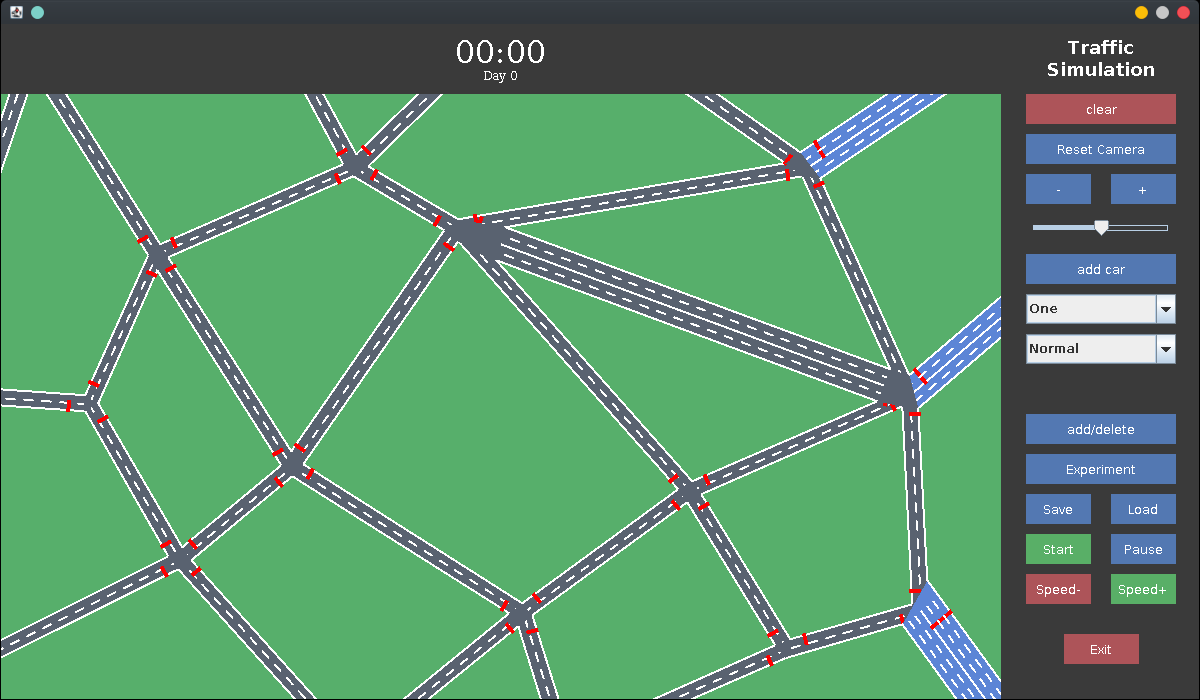
\includegraphics[width=\linewidth]{img/interface.png}
	\caption{Interface of the interactive simulation environment. Different road colors indicate different road types (e.g. streets or highways). \label{fig:interface}}
\end{figure}
	
\subsection{Traffic Flow Simulation}
As mentioned beforehand, the IDM \citep{treiber2000congested} is applied for the simulation of car dynamics. It models traffic flow time- and space-continuous as a combination of \textit{free-road} and \textit{interaction} behaviour. The \textit{free-road term} is governed by a car's intention to reach its desired speed. The acceleration for this behaviour is calculated \citep{treiber2000congested} as

\begin{equation}
	\label{eq:free-road-term}
	\dot{v}_a^{free}(t) = a ( 1 - ( \frac{v_a}{v_0} )^\delta),
\end{equation}

where $a$ refers to a cars maximum acceleration, $v_a$ is its current velocity and $v_0$ the desired velocity. When a car approaches a leading vehicle, it is supposed to slow down in order to avoid collision. This behaviour is modelled by an \textit{interaction term} which incorporates the distance to the leading vehicle and its speed \citep{treiber2000congested}. 

\begin{equation}
	\label{eq:int-term}
	\dot{v}_a^{int}(t) = - a ( \frac{s_0 + v_a T}{s_a} + \frac{v_a \Delta v_a}{2 \sqrt{ab} s_a} )^2
\end{equation}

In the equation above, $s_0$ and $T$ restrict the cars minimum distance in space and time respectively. The interaction term will hence attenuate the free road term when approaching other cars, given by the complete equation for acceleration $\dot{v}(t)$

\begin{equation}
	\dot{v}(t) = \dot{v}_a^{int}(t) + \dot{v}_a^{int}(t)
\end{equation}

In order to simulate a time-continuous model, we need to numerically approximate the integration of the differential equations in \ref{eq:free-road-term} and \ref{eq:int-term}. For that, we choose a small time step $\Delta t$ and repetitively update the velocity as $v(t + \Delta t) = v(t) + \dot{v}(t)$.

\subsection{Traffic Rule Compliance}
Due to the large scale maps used in this work, drivers not only need to behave according to their own desires and other traffic participants. They additionally need to comply to a set of traffic rules as given by speed limits or traffic lights. Following, we briefly discuss the approaches we use in our simulation.

\paragraph{Approaching Traffic Lights} When approaching red traffic lights, drivers will stop in a predefined distance from the intersection, comparable to stop bars in real world streets. Cars that have already exceeded this line will drive through the intersection. 

\paragraph{Speed Limits} The IDM's free road term incorporates a driver's desired velocity as his intended maximum speed. We use an additional parameter, a driver's favoured velocity $v_{fav}$, and determine the desired velocity by taking the minimum of $v_{fav}$ and the roads speed limit.

\subsection{Lane Changing}
In order to incorporate lane changing behaviour into our traffic model, we apply the MOBIL model \citep{treiber2002realistische, kesting2007general}. MOBIL makes decisions for lane changing based on two questions: Is the lane change \textit{incentive} and is it \textit{safe}? The former question is answered based on the potential gain in acceleration on the new lane, while the latter decision is made based on the speed of and distance of the approaching car on the new lane.

\subsection{Arrival Times in a continuous Simulation}
Rather than predefining arrival times for a fixed simulation duration, we dynamically generate inter-arrival times (IAT) during runtime. These IATs are drawn from a predefined distribution independently for each road in the map. Therefore the amount of traffic on a map grows automatically with its size. The IAT can be drawn from the following distributions

\begin{figure}[t]
	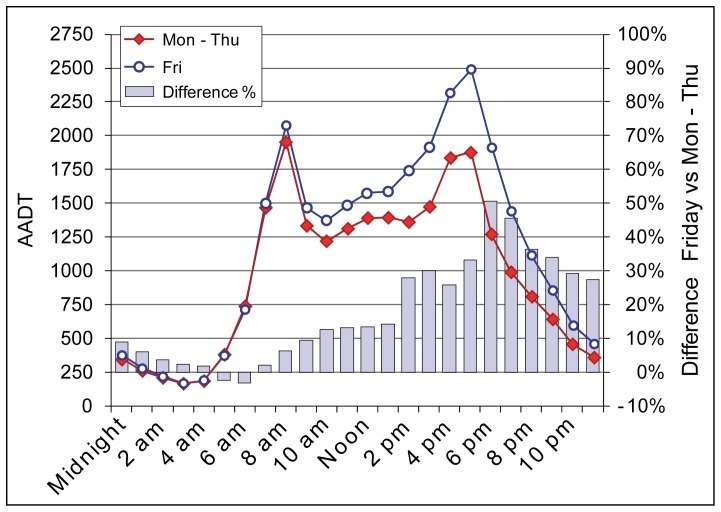
\includegraphics[width=\linewidth]{img/traffic-data.jpeg}
	\caption{Traffic data from the U.S. Department of Transportation. Graphic received from https://www.fhwa.dot.gov/policyinformation/tmguide/
	tmg\_2013/traffic-monitoring-methodologies.cfm \label{fig:traffic-data}}
\end{figure} 
 
\begin{itemize}
	\item Exponential (Poisson Process)
	\item Gaussian
	\item Realistic (Non stationary Poisson Process)
\end{itemize}
 
While the Gaussian and Exponential distribution are standard distributions with adjustable paramters, the realistic distribution is based on real world data from the U.S. Department of Transportation \citep{trafficdata}. We use hourly data and draw IATs based on a poisson process that is then converted to the data using the thinning algorithm by \citet{lewis1979simulation}. The data used is shown in figure \ref{fig:traffic-data}. As can be observed, this creates rush hours around the hours of 8 to 9 am and 5 to 6 pm.

\subsection{Path Finding}
Whenever a car enters the traffic, it needs to get a predefined route to take to its destination. In the simulation, each car runs an instance of a path finding algorithm, two of which were implemented.

\paragraph{A*}
This popular path finding algorithm, based on Dijkstra’s algorithm \citep{dijkstra1959note}, was first introduced in 1968, by \citet{hart1968formal}. It finds the shortest path between the origin and the destination of the cars, given the map only taking the length of the path into account. This is done by using two scores for each node: H and G score. The H score is equal to the Euclidean distance from the node to the destination. The G score is the total distance travelled from the start node to the current node. Based on these two scores, the algorithm finds the shortest path between two points in a graph. 

\paragraph{Advanced A*}
The advanced A* path finding algorithm is very similar to the original version, but it also takes the traffic density and average speed of the roads into account. This is realized by calculating the traffic density and average speed of each road whenever the route of a car is created. The density of a road equals the number of cars on it divided by the length of the road, to get the number of cars per meter of road. The algorithm then adds a weighted density value to the G and H scores of the road to calculate the current best route. The average speed for the roads is taken from the continuously calculated statistics. The value of the average speed is taken away from the score of the road, in order to incentivize the use of roads with a higher speed.

\subsection{Zone-based Scheduling}
Aiming to increase the level of realism, roads on the simulated map have different types of zones that influence the spawn rates and routing of cars. Distinguished zones are \textit{residential}, \textit{mixed}, \textit{commercial} and \textit{industrial}. A road's zone restricts its \textit{available population} in the beginning of the simulation. For instance, commercial zones start with a lower overall population than residential zones. Cars will only spawn from roads as long as there is population available. Whenever a car leaves or arrives at a road, its population is respectively decremented or incremented. Additionally, the zone type determines the traffic flow between different areas of the map. Based on the time of day, cars either mostly move from residential and mixed zones to industrial and commercial zone or vice versa, when they are on their way back home. This way, the simulation also incorporates the difficulties of heavy traffic in one direction, as faced in cities where living and working places are seperated by its different areas. Figure \ref{fig:zone-traffic-flow} sketches how the traffic behaves between the zones based on the time of day.

\begin{figure}
	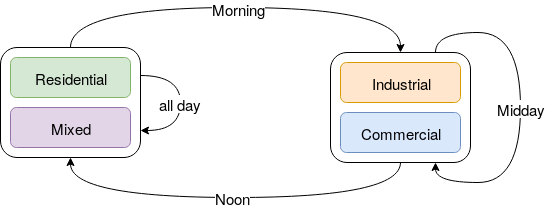
\includegraphics[width=\linewidth]{img/zoned-traffic-flow.png}
	\caption{Traffic Flow between different zone types at different times of the day. \label{fig:zone-traffic-flow}}
\end{figure}

\subsection{Simulation Model}
Putting the above parts together, the simulation procedure depicted by algorithm \ref{alg:simulation} is run.

\DontPrintSemicolon
\setstretch{1.2}
\begin{algorithm}[h]
	\;
	\KwData{Map m, CarList c, Schedule s, days d, delta\_t}
	\;
	\textit{Initialize} trafficlights\;
	\textit{Initialize} tracking variables\;
	\; 
	\While{simulated\_days $<$ d}{
		\textit{update} time\_parameters\;
		\;
		\ForEach{Road r in m}{
			\If{r.nextArrival == now}{
				\textit{spawn} car\;
				r.availablePopulation--\;
				\textit{generate} nextIAT\;
			}		
		}
		\;
		\textit{update} trafficlights\;
		\textit{update} car positions \textit{and} velocities\;
		\textit{remove} arrived\_cars \textit{and} adjust population\;
		\;
		\textit{visualize}\;
		\textit{track} statistics\;
	}
	\;
	\textit{report} statistics\;	
	
	\caption{Simulation procedure. \label{alg:simulation}}

\end{algorithm}
\setstretch{1}

\section{Traffic Control Strategies}

\begin{figure*}[htb]
	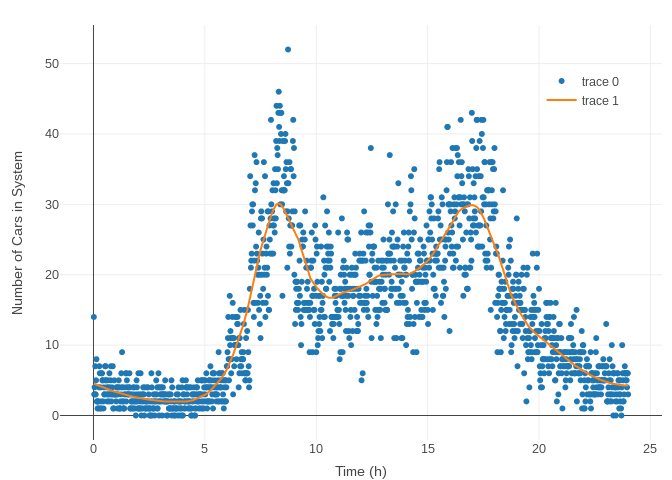
\includegraphics[width=0.5\textwidth]{img/number_of_cars_over_day.png}
	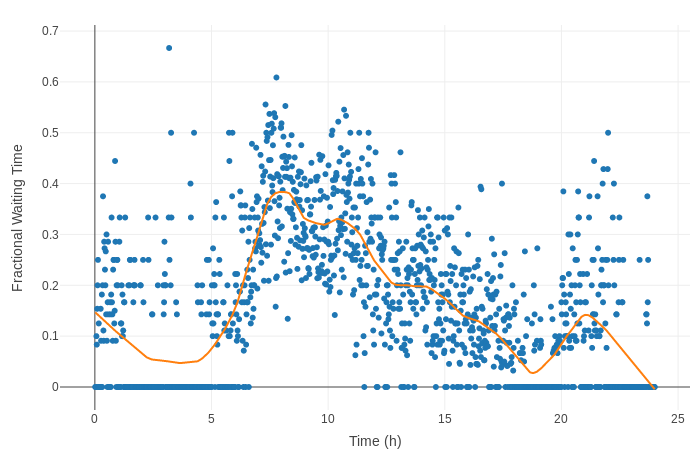
\includegraphics[width=0.5\textwidth]{img/velocity_over_day.png}
	\caption{Number of cars (left) and average velocity of cars (right) in the system simulated for one day. IATs are generated from the empirical distribution shown in figure \ref{fig:traffic-data}. \label{fig:validation}}
\end{figure*}

\label{sec:strategies}
In this section, different traffic control strategies are highlighted as well as their effectiveness in different environments.

\subsection{Benchmark Strategies} 
In order to provide a baseline of what more advanced strategies should be able to outperform, we implemented two simple benchmark strategies. The first one is Basic Cycling, this refers to a traffic light control strategy based on a simple, fixed-time cycle in which one traffic light at a time is green. The second is Informed Cycling refers to a similar strategy, in which a road's green phase is skipped if there are no cars waiting on it. 
Finally, priority Cycling adjusts the green phases linearly based on the density of the roads going into the intersection. 

\subsection{Responsive Strategies}
These strategies should outperform the benchmark strategies as they are more dynamic and change their actions based on their surroundings. The most simple version of such a responsive strategy is priority Cycling,  this strategy adjusts the green phases linearly based on the density of the roads going into the intersection. Weighted Cycling This strategy was chosen to be implemented to reduce the time people spend waiting at a light. Simply put, the traffic lights give priority to those who are waiting at the light, and if no one is waiting, it gives priority to the street with the most cars incoming. This method seems to mimic real-world examples of traffic control systems by acting similar to a traffic light with some form of traffic sensors (pressure plates, traffic cameras, etc.). It also allows the most amount of people possible through fastest, which is extremely effective in situations where a large amount of cars approach from one side. 

\subsection{Advanced Strategies}
The advanced strategies are different from responsive strategies in that they either compare many different inputs to make a decision as to which traffic light should be turned green at which time or they use linear programming. Coordinated traffic lights are traffic lights that exchange information with each other in order to predict future traffic patterns and assure the least amount of congestion possible. Each intersection is outfitted with different types of sensors, depending on the environment in which they are needed. These sensors can include inductive loops, cameras, or microwave radar systems, each of which has its own pros and cons. The coordinated traffic light strategy currently implemented uses features resembling that of a microwave motion sensor. The reason of using this type of sensor is mainly because the detection range can be altered to each one depending on the area it is installed, the ability to accurately detect distance of vehicles, and also it is able to tell if cars are moving towards or away from it. Other reasons for implementing this type of detection system is that in real-world situations, this device can be installed above ground, which greatly reduces cost of installation, and can also be installed very quickly at very low charge and cause minimal traffic disturbance. This type of traffic control system is preferred for areas with minimal obstructions (such as road signs or buildings). Since our current traffic simulation does not have any external obstructions other than cars, this is the best strategy to use. In cases where many obstructions are in play, it would be more recommended to use inductive loops (commonly thought of as ’pressure plates’ installed into the road, but quite costly). The way these microwave motion sensors are used in the simulation is by recognizing how many cars are currently coming towards an intersection from each road and measures the average speed of those cars per road. The road with the lowest average speed will be set to green. If it is close to being a tie than the decision is made by selecting the road with the most amount of cars waiting. In order to prevent certain roads from never turning green, every road has to turn green at least once in a certain amount of time. 

\section{Methodology \& Experiments}
\label{sec:experiments}

\subsection{Measured Statistics}
In order to be able to measure and compare the efficiency of the different strategies applied, various measurements are taken while the simulation is running. One of these is the average speed of the vehicles for each road. Measuring this is done by starting a timer for a car when it enters a road and stopping it when it leaves it. Then, by using the following formula, the average speed is calculated:   

\begin{equation}
	v = \frac{s}{t}
\end{equation}

where $v$ is the velocity, s the road length and t refers to the time spent on a road. Using this, we can also easily derive the average speed on each road. The second statistic measured is the amount of time each car spends waiting at traffic lights. This is achieved by checking at each time step if a car is under a certain speed and is not accelerating. Whenever the previous conditions are fulfilled, the total amount of waiting time is increased by the size of the time step. The purpose of the control strategies is to maximize the average speeds and minimize the time spent waiting in congestions.

\subsection{Simulated Maps}

\subsection{Simulation Validation}
In order to validate both the IA generation as well as the general behaviour of different measures and dynamics, we validated the simulation environment using the average speed of cars, their number on the map as well as fractional waiting times in the simulation as a development over one day. Figure \ref{fig:validation} shows the results in three graphs. As can be observed, not only the density, but also both other dependent measures resemble the rush hour pattern from the original data.<

\subsection{Methodology}
It is the objective of this work to compare multiple systems (i.e. strategies) under different conditions. Since it is desirable in such a setting to not only compare these systems with a baseline or benchmark system but rather rank them by performance, a convenient framework for such a comparison is needed. An all-pairwise comparison is not desirable, since the total of 6 systems would require 30 comparisons, which would result in tiny confidence levels due to Bonferroni inequality \citep[see e.g.][]{law2007simulation}. Instead, the sample size required for each system in order to achieve a confidence level of $\alpha$ for the complete ranking can be determined by the approach of \citet{dudewicz1975allocation}. In order to perform statistical calculations on the data, it is often necessary but at least useful to have IID observations. It is obvious that this independence can not be assumed in a traffic simulation between individual cars, since the delay of one car often influences that of others in shared roads and queues. While restarting the simulation $n$ times in order to get $n$ observations that can be combined to a grand mean seems an obvious choice, the day-based simulation also allows to run multiple days and assume independence between days, since traffic is supposed to somewhat reset during night.

Since this is a non-terminating simulation, it is furthermore necessary to take a so called \textit{warm-up period} or \textit{transient phase} into account. It is the result of starting the simulation in an initial state that might not represent an actual state of the simulation in steady-state or inside a cycle. Therefore, the period where the simulation enters the steady-state needs to be removed from any statistical calculation such that it does not bias their results to the initial situation. Arguably, simulating traffic on the basis of days results in a cyclic simulation. Importantly though, this will not necessarily mean that the simulation entirely resets to zero cars in the system at midnight. For those reasons and the sake of convenience, in any experiment, the first simulated day will be removed from the simulation.

\section{Results}
\label{sec:results}

\section{Discussion}
\label{sec:discussion}

\section{Conclusion}
\label{sec:conclusion}

%- Often times, better road layout makes way more of a difference than different strategies (tiefighter example)

{\tiny\printbibliography}

\end{document}